\documentclass[14pt]{article}
\usepackage[utf8]{inputenc}
%\documentclass[11pt,letterpaper,dvips]{article}
%author: David DeMuth, Jr. Fall 2016 - written using Overleaf
\usepackage{tikz}
\usetikzlibrary{arrows}
\usepackage{verbatim}
\usepackage{tkz-euclide}
\usetikzlibrary{shapes.callouts}
\usetikzlibrary{decorations.pathmorphing,patterns}  %needed for spring 
\usetikzlibrary{positioning,decorations.markings,arrows.meta}
\usetikzlibrary{calc,patterns,angles,quotes}

\usepackage{amsmath}
\usepackage{graphicx}
\usepackage{tabularx}
\usepackage{epsfig}
%\usepackage{pgfkeys}
\usetikzlibrary{matrix}
\usepackage{epsfig,wrapfig} 
%\usepackage{tabularx}
%\usepackage{adjustbox}
\usepackage{enumerate}
\usepackage{enumitem}  %itemsep
\usepackage{array}
\usepackage{multicol}
\usepackage{multirow}
\usepackage{caption}
\usepackage{diagbox}   %\usepackage{slashbox}  
\usepackage{url}
\usepackage{pgfplots}

%\usepackage []{accessibility}
%\usepackage[tagged]{accessibility}
%\usepackage{axessibility}
\usepackage{pdfcomment}

%see https://en.wikibooks.org/wiki/LaTeX/Page_Layout#Customizing_with_fancyhdr
\usepackage{fancyhdr}
\pagestyle{fancy}
\fancyhf{}
\lhead{Physics Laboratory}
\rhead{Page \thepage}
%\setlength{\headheight}{15.2pt}
\renewcommand{\headrulewidth}{1pt}
\fancyhfoffset[L]{6mm}% slightly less than 0.25in
\fancyhfoffset[R]{6mm}%
%\fancyhead[L]{\thepage\hskip3mm\vrule\hskip3mm\leftmark}%
%\fancyhead[R]{\rightmark\hskip3mm\vrule\hskip3mm\thepage}%
%\fancyfoot[C]{Confidential} ??

%\setlength{\textwidth}{7.25in}\setlength{\textheight}{10in}
\setlength{\parskip}{5pt}
\setlength{\parindent}{0pt}
\setlength{\topmargin}{-4.5in}
\setlength{\textheight}{23.5cm}
\setlength{\textwidth}{17cm}
\setlength{\oddsidemargin}{-0.5cm} 
\setlength{\evensidemargin}{-0.5cm}
%\setlength{\hyphenpenalty}{9500}

\renewcommand{\baselinestretch}{1.02} %units?
\newcommand{\degr}{^\circ}

\renewcommand{\section}[1]{\vspace{6pt} \noindent\mbox{#1} \newline \noindent}
\renewcommand{\subsection}[1]{\vspace{6pt} \noindent\mbox{\underline{#1}} \newline \noindent}
\renewcommand{\subsubsection}[1]{\vspace{6pt} \noindent\mbox{\underline{#1}}\noindent}
\renewcommand\figurename{\it Fig.}

\newfont{\sansb}{cmssbx10}
\newfont{\sans}{cmss10}
\newfont{\tablefont}{cmsl12}

\voffset=0pt
\setlength{\topmargin}{0pt}
\setlength{\headsep}{0pt}
%\special{pdf: pagesize width 8.5in height 11in}

%\def \nameline {\hfill NAME:\hbox to 200pt{\hrulefill}\medskip} %see below                    %\nameline
\def \courseno {212}
%\title{\Physics \courseno~ Lab 7: Statics and Torque}
%\author{David DeMuth, Jr.}
%\date{\today}
%\newfont{\eightrm}{cmr8}
%\newfont{\boldbigtenrm}{cmbx10 scaled\magstep1}
%\newfont{\boldtenrm}{cmbx10}

\newcommand{\heading}[1]{{\boldbigtenrm #1}}
\newcommand{\subheading}[1]{{\boldtenrm #1}}
\newcommand{\referencepages}[1]{\vskip -25pt{\eightrm REFERENCE: #1}}
\newcommand{\materials}[1]{\vskip -15pt{\eightrm MATERIALS: #1}}
%\def \version{\nopagenumbers \hbox to \hsize{\vbox to 0pt{\vskip-2.5pt \hfil {{\eightrm Physics 161 Version \today}}\hfil}}}

\font \eightrm=cmr8
\font \tenrm=cmr10
%\font\smallheadfont=cmr8 at 8 truept
%\font\nicefont=cmss10 scaled\magstep2
%\font\smallnicefont=cmss10 at 9truept
\font \boldtenrm=cmbx10
%\font \boldbigtenrm=cmbx10 scaled\magstep1
%\font \bigtenrm=cmr10 scaled\magstep2

\def\newline{\hfill\penalty -10000}  % Use to force a line break, if needed.                                                                                                                 
\def \ln#1{\newline{#1}}
\def \blankpage#1{\newpage\nameline \newline {\bf Problem \# {#1} (Cont'd)}}
\def \setheadline#1{\footline{}\headline={\hfill {\eightrm #1 p. \folio}}}
\def \normbs {\baselineskip 11pt}
\def \specbs {\baselineskip 14pt}
\def \nques#1#2{\normbs \medskip \smallitem {#1)} {#2} \specbs}
\def \nlist#1#2{\smallitem (\hskip 2pt) {#1)} \hskip 10pt {#2}\leftskip 0pt}
\def \version{\nopagenumbers \hbox to \hsize{\vbox to 0pt{\vskip-2.5pt \hfil {{\eightrm Physics 212 Version \today}}\hfil}}}
%http://library.caltech.edu/coda/theses/latex-quickguide.pdf 
\begin{document}
\thispagestyle{plain} %empty, plain
%\pagenumbering{alph} %roman
\baselineskip 14pt

\def \headline{\hfill {NAME:\hbox to 180pt{\hrulefill}}}
\def \footline={20230130}%{20161017}
\def \setheadline#1{\footline{}\headline={\hfill {\eightrm #1 p. \folio}}}
\vskip 0pt  \headline

\referencepages{College Physics: Chapter 16}
%\materials{Styrofoam cups with lid, aluminum and iron balls, pennies, thermometer, hotplate}

\newcount \questionno
\newcount \sumquestions \sumquestions=0
\def \question#1{\advance\questionno by 1{\bf Question~\number\questionno:}{\global\advance\sumquestions by #1} }
\def \showsumquestions{\immediate \write0 {>>> Sum of questions >>> \number\sumquestions pts}}

\def \degc{$^oC$}

{\bf Physics \courseno~ Laboratory: Vibrations and Sound}

\subheading{Warm up Exercises~} 

A mass loaded spring hanging vertically can be set into periodic motion. A mass attached to the end of string will also swing in a regular way.  In the laboratory we study the periodic motion of springs and pendula.

{\bf Question 1:} When a $100~g$ ($0.1~kg)$ mass is attached to a spring which hangs vertically, it stretches by $\triangle y=2.5~cm$. A restoring force $F_R$ caused by the stretched spring depends on the stiffness of the spring $k$ and the displacement ($\triangle y$) from the springs equilibrium position; $F_R=-k\triangle y$ (Hooke's Law). Use the diagram below to form a relationship between the weight $W$ and $F_R$ for the static case. Using Hooke's Law, determine the stiffness $k$ of the spring for a static case.  %How would you calculate the period of a mass-spring system if set into motion? %\vskip 5pt

%\centerline{\psfig{file=figs/lesson15_spring1.ps,height=80pt,bbllx=22bp,bblly=655bp,bburx=442bp,bbury=774bp}}
%\begin{figure}[h]
%\centering
%\includegraphics[width=0.7\textwidth]{figs/lesson15_spring1.png}
%\end{figure}

\begin{figure}[h]
\centering
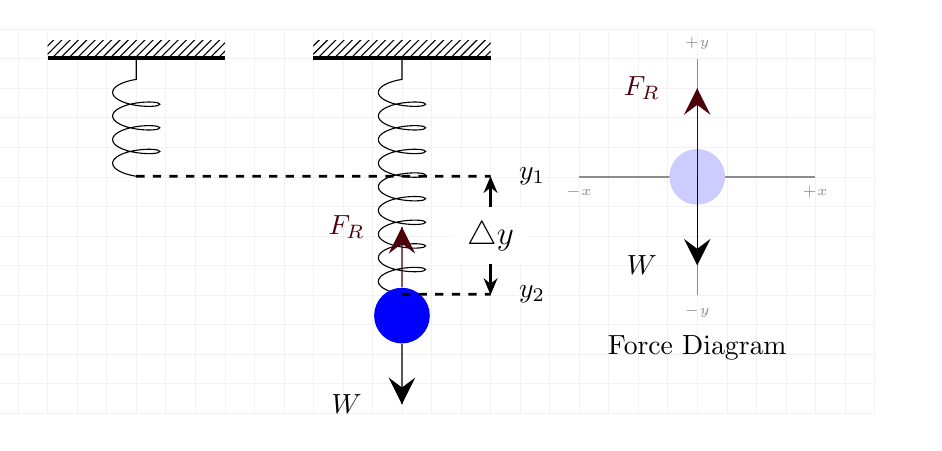
\begin{tikzpicture}[scale=0.75]  %scale adjustment requires re-values
    \draw[step=.5, lightgray!20, very thin] (0,0) grid ++(15.0,6.5);  %edit grid - to hide set lightgray!0
    \definecolor{object-vr}{RGB}{76,0,09};  %red  
    
    \def\xo{1.00};             \def\yo{6.01};            %set box origin x,y
    \def\dx{3.0};              \def\dy{0.3}; %set box horizontal width, vertical height
    \def\bllx{\xo};            \def\blly{\yo};
    \def\burx{\xo+\dx};        \def\bury{\yo+\dy};
    \coordinate(ALL) at (\bllx,\blly);   %total box lower left coordinate
    \coordinate(AUR) at (\burx,\bury);   %total box upper right
    \fill [pattern = north east lines] (ALL) rectangle (AUR);
    \draw[ultra thick] (\bllx,\yo) -- (\burx,\yo);
    \coordinate(aa) at (\xo+\dx/2,\yo);
    \coordinate(ab) at (\xo+\dx/2,\yo-2);
    \draw[decoration={aspect=0.3, segment length=3mm, amplitude=3mm,coil},decorate] (ab) -- (aa); 

    \def\xo{5.50};             \def\yo{6.01};            %set box origin x,y
    \def\dx{3.0};              \def\dy{0.3}; %set box horizontal width, vertical height
    \def\bllx{\xo};            \def\blly{\yo};
    \def\burx{\xo+\dx};        \def\bury{\yo+\dy};
    \coordinate(BLL) at (\bllx,\blly);   %total box lower left coordinate
    \coordinate(BUR) at (\burx,\bury);   %total box upper right
    \fill [pattern = north east lines] (BLL) rectangle (BUR);
    \draw[ultra thick] (\bllx,\yo) -- (\burx,\yo);
    \coordinate(ba) at (\xo+\dx/2,\yo);
    \coordinate(bb) at (\xo+\dx/2,\yo-4);
    \draw[decoration={aspect=0.3, segment length=3mm, amplitude=3mm,coil},decorate] (bb) -- (ba); 
    \node[circle,fill=blue,inner sep=2.5mm] (bc) at (\xo+\dx/2,1.65) {};

    \draw[line width=1.0,dashed] (ab) -- (\xo+\dx,\yo-2)  node[at end, xshift=15pt]{$y_1$}; 
    \draw[line width=1.0,dashed] (bb) -- (\xo+\dx,\yo-4) node[at end, xshift=15pt]{$y_2$}; 
    \draw[line width=1.0,black,{Stealth[scale=0.8,angle'=45]}-{Stealth[scale=0.8,angle'=45]}] (\xo+\dx,2)--(\xo+\dx,\yo-2);
    \tikzstyle{ann} = [fill=white,font=\large,inner sep=5pt]
    \node[ann] at (\xo+\dx,3) {$\triangle y$};
     
\draw [decoration={markings,mark=at position 1 with
    {\arrow[object-vr,scale=3,>=stealth]{>}}},postaction={decorate},object-vr] (bc) -- ++(0,+1.5) node[at end,xshift=-20pt] {$F_R$};
        
\draw [decoration={markings,mark=at position 1 with
    {\arrow[scale=3,>=stealth]{>}}},postaction={decorate}] (bc) -- ++(0,-1.5) node[at end,xshift=-20pt] {$W$};
     
\coordinate(O) at (12,4); 
\draw[line width=0.5,gray!90] (O) -- ++(-2,0) node[at end, below]{\tiny $-x$};
\draw[line width=0.5,gray!90] (O) -- ++(+2,0) node[at end, below]{\tiny $+x$};
\draw[line width=0.5,gray!90] (O) -- ++(0,+2) node[at end, above]{\tiny $+y$};
\draw[line width=0.5,gray!90] (O) -- ++(0,-2) node[at end, below]{\tiny $-y$};
          
\node[circle,fill=blue!20,inner sep=2.5mm] at (O) {};
\node[black] at (12,1.1) {Force Diagram};

\draw [decoration={markings,mark=at position 1 with
    {\arrow[object-vr,scale=3,>=stealth]{>}}},postaction={decorate},object-vr] (O) -- ++(0,+1.5) node[at end,xshift=-20pt] {$F_R$};
        
\draw [decoration={markings,mark=at position 1 with
    {\arrow[scale=3,>=stealth]{>}}},postaction={decorate}] (O) -- ++(0,-1.5) node[at end,xshift=-20pt] {$W$};
\end{tikzpicture}
\caption{Scenario view and Force Diagram for a static mass loaded spring.} \label{fig:figure1}
\end{figure}

\vskip 5pt

{\bf Question 2:} A spring's stiffness is more reliably determined from multiple measurements and by determining the slope of the line that fits a weight versus displacement scatter plot graph. Masses of 0.0, 0.2, 0.4, 0.6, 0.8, and 0.1 kg are suspended one at a time on a spring of unknown stiffness. Correspondingly vertical displacements of 0.00, 0.05, 0.10, 0.15, 0.20, and 0.25 m are realized. Plot $mg~(N)$ vs. $\Delta y~(m)$ to determine the stiffness $k$.
%https://docs.google.com/spreadsheets/d/1Zma3XB8F9_aYSmhIbrfjl0-AE8qSFNDc4iZtPQXoFIc/edit?usp=sharing

\vskip 100pt

{\bf Question 3:} A mass loaded spring completes $12~cycles$ in $10~seconds$, what is its frequency and period?\vskip 60pt

{\bf Question 4:} A $100~g$ mass is attached to a spring hanging vertically and set into motion. Using the spring constant $k$ that was calculated in Question 2, determine the period (in $s$) of the motion? What is its frequency?\vskip 0pt

%{\bf Question 4:} If a pendulum completes $24~cycles$ in $30~seconds$, what is its period and frequency?
%\vskip 60pt

%{\bf Question 5:} What is the period of a pendulum whose length is $10~meters$?\vskip 0pt
\newpage 
\vphantom{}

\subheading{Spring Experiments:} You will explore the relationships among a spring having stiffness $k$, a suspended mass $m$, and the period $T$ of an oscillating mass loaded spring by utilizing the PHET Masses and Springs simulation: 
\vskip 0pt
\centerline{\url{https://phet.colorado.edu/en/simulation/masses-and-springs}}

\vskip -5pt
\begin{wrapfigure}{l}{0.12\textwidth}
    \centering
    \pdftooltip{\includegraphics[width=18mm]{figs/PHET-mass-and-spring-mass-icon-lab1.png}}{PHET Lab Icon}%\usepackage{pdfcomment}
    %\caption{PHET Icon}
    \label{fig:labicon}
\end{wrapfigure}

%In this activity you are asked to explore a relationship between the weight of a mass attached to a spring and the spring's "balancing" force.  

The startup screen of the PHET Masses and Springs simulation has four modes: select the``Lab'' tab to discover a vertical spring with adjustable mass and spring constant controls (see Fig. \ref{fig:phet-mass-and-spring-lab-1}). %There you'll discover a feature-full simulation with several components.

Firstly, pick a spring by assigning a ``stiffness'' via the Spring Constant 1 slider by selecting a ``tic'' mark of your choice.  The position of the slider are counted as tics counted from the Small (tic 1) slider indent. There are ten tic slider locations (1-10) in total. 

With a spring's stiffness declared, the goal is to determine the spring constant. Use the ruler tool to measure the vertical stretch of the spring for several loads; see Table \ref{tab:hookeslaw} for a spreadsheet table design. 

%and is to be cast into a spreadsheet. Report your spring constant tic mark in your spreadsheet.

%\begin{minipage}{0.55\textwidth} 
%Experiment with two different springs, those having a particular spring constant which is selected by the slider, report the spring in tics counted from the Small (tic 1) indent, e.g. you might select the spring at tic 3, and a second at tic 6. There are 10 tic location in total. The same springs you select will be used later on in this lab. \vspace{5mm}
%
%Notice also the Damping option, setting it to "Lots" so that you do not have to wait for the spring to oscillate to a motionless position. There is also a movable line feature that can be used as a reference when measuring vertical displacement.
%
%    \vspace{0pt}
%\end{minipage}
%    \hspace{0pt}
%\begin{minipage}{0.40\textwidth}
%    \centering
%\includegraphics[width=0.8\textwidth]{figs/PHET-mass-and-spring-lab-1.png}
%\vspace{0pt}
%\end{minipage}
\begin{wrapfigure}{r}{0.45\textwidth}
    \centering
    \pdftooltip{\includegraphics[width=0.39\textwidth]{figs/PHET-mass-and-spring-lab-1.png}}{PHET Lab}
    \caption{PHET Masses and Springs Lab}
    \label{fig:phet-mass-and-spring-lab-1}
\end{wrapfigure}

To mark the position of your bare spring, grab the ``Movable Line'' laser from the tools pane, and locate the red dashed line of the laser at the bottom of the non-mass loaded spring. This will be your reference line each time you load the spring with a mass pendent; load the spring with the $100~g$ mass selected from the bottom of the screen.  The mass of the pendant is adjustable via the Mass slider, these ranging from $50$ to $300$ grams.  For a selected mass, starting with $0~g$, record it's mass in $grams$ to your spreadsheet; add a column that reports mass in $kg$ using a formula to calculate $kg$ from $g$. For each mass, determine the object's weight in $Newtons$ in an adjacent column. 

Notice the Damping option, setting it to ``Lots'' so you do not have to wait for the spring to oscillate to a motionless state. Use the meter stick tool to measure the associated displacement, and report the displacement to your spreadsheet data table in $cm$. Use formula to generate a displacement in $meters$ column.

Complete at least six measurements. From this data create a scatter plot graph for the pendent weight in $Newtons$ versus vertical displacement in $m$, adding trend line, equation, and $R^2$ fit value. What does the slope of your scatter plot represent?

%Optional: Repeat the activity for a second spring with a significantly different spring constant.

\newcolumntype{L}[1]{>{\raggedright\let\newline\\\arraybackslash\hspace{0pt}}m{#1}}  %define column width
\newcolumntype{C}[1]{>{\centering\let\newline\\\arraybackslash\hspace{0pt}}m{#1}}
\newcolumntype{R}[1]{>{\raggedleft\let\newline\\\arraybackslash\hspace{0pt}}m{#1}}
\renewcommand{\arraystretch}{1.1}  %adjust row height

\begin{table}[b]
\centering
\captionsetup{width=0.8\textwidth}
\caption{Experiment Data Table} \label{tab:hookeslaw}
\begin{tabular}{|C{1.4cm}|C{1.4cm}|C{1.8cm}|C{1.8cm}|C{2.1cm}|C{2.1cm}|C{2.1cm}|} \hline 
%
Spring & Tic Mark & Mass ($g$) & Mass ($kg$) & Weight ($N$) & Displacement ($cm$) & Displacement ($m$)   \\ \hline
 1 &  & 0  &0&0&0&0 \\ \hline
 1 &  & 50 & & & &  \\ \hline
 1 &  &100 & & & &  \\ \hline
 1 &  &150 & & & &  \\ \hline
 1 &  &300 & & & &  \\ \hline
 1 &  &250 & & & &  \\ \hline
 1 &  &300 & & & &  \\ \hline
 %2 & & & & & &  \\ \hline
 %2 & & & & & &  \\ \hline
 %2 & & & & & &  \\ \hline
 %2 & & & & & &  \\ \hline
 %2 & & & & & &  \\ \hline
\end{tabular}
\end{table}
%example spreadsheet: https://docs.google.com/spreadsheets/d/1Zma3XB8F9_aYSmhIbrfjl0-AE8qSFNDc4iZtPQXoFIc/edit#gid=0

%Report your determinations of spring constants for the two spring you selected here.

\newpage
\vphantom{}

\subheading{Investigating Amplitude}: In the previous section you explored the relationship between mass, weight and equivalently the restoring force $F_R$, with the vertical displacement $\Delta y$ to discover a spring's spring constant $k$.  

In comparing springs, those with increased $k$ are stiffer, and become harder to stretch (or compress). That is to say, the restoring force of a spring depends upon the properties of the spring; is it metal or plastic, is it of a small or large diameter, et cetera. Notice in the PHET simulation springs seem to "bulk up" when moving the Spring Constant 1 slider to a larger value (see Fig. \ref{fig:kslider}).

\begin{wrapfigure}{r}{0.25\textwidth}
    \centering
    \pdftooltip{\includegraphics[width=40mm]{figs/PHET-mass-and-spring-k-slider1.png}}{The spring constant is adjusted via PHET app.}%\usepackage{pdfcomment}
    \caption{PHET Slider}
   \label{fig:kslider}
\end{wrapfigure}

All of your Hooke's Law exploration was for a static situation; a motionless mass was supported by a spring. Here we will instead explore how a suspended mass will move stretched to an initial ``amplitude'' and released.

From the previous experiment, you determined the spring constant for one spring.  Using that same spring setting (tic mark on the slider), suspend a $50~g$ mass, pull it down some distance (amplitude), and release it, what happens?  Is the situation to fast to monitor?  Compare the motion with a $250~g$ load; explore ``Damping.''

\begin{wrapfigure}{r}{0.25\textwidth}
    \centering
    \pdftooltip{\includegraphics[width=40mm]{figs/PHET-mass-and-spring-tools1.png}}{The spring constant is adjusted via PHET app.}%\usepackage{pdfcomment}
    \caption{PHET Tools}
   \label{fig:tools}
\end{wrapfigure}

Curious is the effect of your choice of amplitude. That is, does your choice for the initial vertical displacement have any bearing on the period of the motion; again the initial vertical displacement is the ``amplitude'' of the oscillatory motion.  The ``period'' of the motion of an oscillating spring mass system is given as the time to complete one cycle. A cycle could be starting at the equilibrium position, to the top of the motion, back through the equilibrium on to the bottom of the motion, then back to the equilibrium.

The PHET simulation has tools (Fig. \ref{fig:tools}) to grab: the ruler, the stopwatch, the movable line, and the mass equilibrium line. The equilibrium line is the indicator where when motionless, its center of the mass is identified. %That it a good reference of the period measurement. 

Adjust the ``Damping'' slider to None. While not realistic, without damping we can better probe the relationship between amplitude and period.

Set the mass into motion after stretching it some distance, say $20~cm$. We say then that the amplitude of the motion will then be $20~cm$.  Measure the corresponding period but not for just one cycle, but rather for 10 cycles.  The period of the motion is then the stopwatch measurement divided by 10 cycles. You might experiment with the Slow (motion) button.

Ultimately you want to comment on how the amplitude affects the period.  An example data table design is provided in Table \ref{tab:tabletwo}.

\begin{table}[h]
\centering
\captionsetup{width=0.8\textwidth}
\caption{Experimental data for spring constant $k=$ \hbox to 30pt{\hrulefill} $N/m$.} \label{tab:tabletwo}
\begin{tabular}{|C{1.1cm}|C{1.1cm}|C{1.1cm}|C{1.1cm}|C{1.1cm}|C{1.1cm}|C{1.1cm}|C{1.1cm}|C{1.1cm}|C{1.1cm}|C{1.1cm}|} \hline 
%
Spring & Tic & Mass $g$ & Mass ($kg$) & Weight ($N$) & $\Delta y$ ($cm$) & $\Delta y$ ($m$) & $T_1$ ($s$) &$T_2$ ($s$)&$T_3$ ($s$) &$T_{ave.}$ ($s$)\\ \hline
 1 & &  & & & &&&&&  \\ \hline
 1 & &  & & & &&&&&  \\ \hline
 1 & &  & & & &&&&&  \\ \hline
 1 & &  & & & &&&&&  \\ \hline
 1 & &  & & & &&&&&  \\ \hline
\end{tabular}
\end{table}

Create scatter plots for period (in seconds) versus amplitude for each spring and mass you explore, as many as are enough to convince yourself on what the effect of varying the amplitude is on the period of the motion.

\newpage
\vphantom{}

\subheading{Investigating Mass}: You now have a sense on how the amplitude for a spring affects the period.  Now we will pursue the effect of varying the mass of the suspended object.

Using the same PHET simulation, and the same spring that was used in the previous experiment, let's vary the mass.  Try at least five masses, suggesting in the range of $50-250~g$. 

For each suspended mass, again with Damping off, pull the mass down to a desirable amplitude, then release the mass to watch it oscillate. Measure the time to complete five cycles, then the time to complete one cycle.  Repeat this measurement for a total of five different masses. For each mass, repeat the measurement twice to ensure precision.  Table \ref{tab:tablethree} provides data table guidance.

\begin{table}[h]
\centering
\captionsetup{width=0.8\textwidth}
\caption{Experimental data for spring constant $k=$ \hbox to 30pt{\hrulefill} $N/m$.} \label{tab:tablethree}
\begin{tabular}{|C{1.0cm}|C{0.8cm}|C{1.1cm}|C{1.1cm}|C{1.1cm}|C{1.0cm}|C{1.0cm}|C{1.0cm}|C{1.0cm}|C{1.0cm}|C{1.0cm}|C{0.6cm}|} \hline 
%
Spring & Tic & Mass ($g$) & Mass ($kg$) & Weight ($N$) & $\Delta y$ ($cm$) & $\Delta y$ ($m$) & $T_1$ ($s$) &$T_2$ ($s$)&$T_3$ ($s$) &$T_{ave.}$ ($s$) & ?\\ \hline
 1 & & 50  & & & &&&&&&  \\ \hline
 1 & & 100 & & & &&&&&&  \\ \hline
 1 & & 150 & & & &&&&&&  \\ \hline
 1 & & 200 & & & &&&&&&  \\ \hline
 1 & & 250 & & & &&&&&&  \\ \hline
\end{tabular}
\end{table}

Create a scatter plot graph of period in seconds versus mass in kilograms.  Is this a direct relationship?  What is the value of the $R^2$-value for the fitted trend line?  If its not a great fit to a line, can you improve that fit somehow?  Could somehow the slope of the Period-vs-Mass graph have some physical significance?  

If you were to instead run this experiment on the Moon or another planet, would you get the same results?

%\newpage 
%\vphantom{}

\subheading{Pendulum Experiments}: A pendulum is a body suspended from a fixed point so that it can be set into motion to swing freely.  Through experiment the period of a pendulum will be determined % is given by $T=2\pi\sqrt{l\over g}$.
using the simulation: \url{https://phet.colorado.edu/en/simulation/pendulum-lab}.

\begin{wrapfigure}{r}{0.45\textwidth}
    \centering
    \pdftooltip{\includegraphics[width=75mm]{figs/PHET-pendulum-sim.png}}{PHET Pendulum App}%\usepackage{pdfcomment}
    \caption{PHET Pendula}
   \label{fig:pendula}
\end{wrapfigure}

In a way similar to our approach with the vertical spring,  determine answers to the following questions: 1) How does the amplitude affect the period of the motion? 2) How does the mass of the pendulum bob affect the period of the motion?  3) How does the length of the cord affect the period of the motion? 4) If you ran the experiment on the Moon, Mars, or Jupiter, would the period change, how?  

Design experiments using the PHET simulation. For each question, a data table will be required, multiple trials, and scatterplots for 1) Period vs. Amplitude, 2) Period vs. Mass, 3) Period vs. Length, and 4) Period vs. Planetary Gravity.  Formulate a mathematical relationship that expresses the Period $T$ with any of these parameters, including any proportionality constants.

The associated data tables and scatter plots should be included as additional will be uploaded on the Blackboard site as an assignment.  The best work will include descriptions of procedures and findings.

\newpage
\vphantom{}

\subheading{Homework: Measuring the Stiffness of the Coil Springs of a Car}

Coil springs and shock absorbers are used to soften and dampen the oscillatory motion that is experienced when driving in a truck or car on a road that is not perfectly level. 

As the front left tire/wheel of a moving truck encounters a pothole, for example, the wheel plummets into the hole as does the rest of that section of the car. As abruptly, the front tire then is forced upwards as it exits. 

Stiff coil springs are used to absorb some of the energy of the blow while shock absorbers in turn dampen the vibrations of the coil spring to only a few oscillations.  Without a functioning shock absorber, the spring will oscillating numerous times before damping.

\begin{wrapfigure}{r}{0.45\textwidth}
    \centering
    \pdftooltip{\includegraphics[width=75mm]{figs/truck-coil-and-shock.png}}{Shock Absorber on Display}%\usepackage{pdfcomment}
    \caption{A coil spring and shock absorber viewed from under a truck.}
   \label{fig:truck-coil-and-shock}
\end{wrapfigure}
%image reference: https://cdn.shopify.com/s/files/1/0267/8256/4539/products/images_ePIM_original_9110_super-duty-4-link_installed_w715_h500_q80_c5bc6c35-3694-4170-bdd7-12823bc70848_500x.jpg?v=1663015489

The goal of this activity is to measure the spring constant of the front coil springs on a truck or car. To to this,
you will need a group of 4-6 persons, and a meter stick. 

On level ground, measure the height of the bottom of the bumper or some other fixed point of the front of a vehicle. Then measure the vertical displacement at that same point as one, two, three, ... persons are asked to stand on the bumper. Be sure that the load is distributed evenly, that is balanced at the center of the bumper. 

Record the weight of each person, and the vertical displacement in a spreadsheet table.

Also record the height as each person is removed from the bumper, then using the same height with
that measured in the loading phase, calculate an average vertical displacement in your spreadsheet.

Determine the effective spring constant for the front of the car. Note that you are measuring the spring constant of two parallel springs, and likely either the shocks or struts which serve to dampen the oscillatory motion. If curious, consult the text or other references on how the spring constants for two springs can be decoupled into each spring.

Write a short report discussing this experiment and your findings. Include a sketch, free-body and force diagram as well as a table of your data. Include a picture of your crew while loading the bumper.



\newpage 

\vphantom{test}

\subheading{Measuring the Velocity of Sound in Air:~}
Standing waves can form in a pipe which is open to the air at one end and closed at the other end when the chamber length $L$ and the wavelength of the source are related as $L_n=\frac{n}{4}\lambda$ where $n=1,3,5,..$ which correspond to the fundamental frequency $n=1$, the first harmonic frequency, etc.  If you place a vibrating tuning fork near the open end of the pipe and adjust the chamber length, eventually you can find the resonance points.

%\centerline{\psfig{file=figs/sound_apparatus.ps,height=110pt,bbllx=10bp,bblly=570bp,bburx=500bp,bbury=780bp}}

\begin{figure}[h]
\centering
\includegraphics[width=0.6\textwidth]{figs/sound_apparatus.png}
\end{figure}

\subheading{\bf Exploration:~}
Explore finding the first resonant point for one of the tuning forks provided by slowly varying the chamber length.
When you reach a resonant point, the intensity of the sound will increase dramatically.

\subheading{\bf Prediction:~}
The precise location of each resonant point can be predicted. 
Given the frequency of the tuning fork, the corresponding wavelength is determined from the relationship $v=f\lambda$ where $f$ and $\lambda$ are the frequency and wavelength of the tuning fork and  $v$ is the velocity of sound. The accepted value for the velocity of sound in air depends on the temperature $v_T = v_0 \sqrt\frac{T}{T_0}$ where $v_T$ is the velocity of sound at a temperature $T$ (measured in Kelvins), and $v_0$ is the velocity of sound in air at a temperature of 20\degc. Measure the temperature of the room and calculate the accepted velocity of sound in air.

\vskip 80pt

Predict the resonant points corresponding to the fundamental ($L_1$), first ($L_2$) and second harmonic frequencies for each of the tuning forks provided. Record these in Table \ref{tab:table9}.

%%\vskip 80pt
%\vskip 5pt\thicksize=1.5pt\thinsize=0.6pt %default
%%\noncenteredtables
%\begintable
%\multispan4{\tstrut\hfill\quad \bf TABLE IX: RESONANCE LENGTH PREDICTIONS \quad\hfill}\cr
% | \bf Fork 1: \hskip 25pt Hz | \bf Fork 2: \hskip 25pt Hz | \bf Fork 3: \hskip 25pt Hz \cr
%\entry{$L_1$} | | | \cr
%\entry{$L_2$} | | | \cr
%\entry{$L_3$} | | | \endtable

\begin{table}[h]
\centering
\captionsetup{width=0.8\textwidth}
\caption{Resonance Length Predictions} \label{tab:table9}
\begin{tabular}{|C{0.7cm}|C{0.7cm}|C{2.9cm}|C{2.9cm}|C{2.9cm}|} \hline 
& & \bf Fork 1: \hskip 25pt Hz & \bf Fork 2: \hskip 25pt Hz & \bf Fork 3: \hskip 25pt Hz \\ \hline
& $L_1$ & & & \\ \hline
& $L_2$ & & &  \\ \hline
& $L_3$ & & &  \\ \hline  
\end{tabular}
\end{table}

\newpage
\vphantom{}

\subheading{\bf Experiment}

{\bf Question 5} Using your predictions for the resonance points as starting points, adjust the piston of the sound tube so that the chamber is at the prescribed depth. Set the associated tuning fork into vibration and determine as accurately as possible the resonant points. Record these below. 

\begin{table}[h]
\centering
\captionsetup{width=0.8\textwidth}
\caption{Experimental Data} \label{tab:table10}
\begin{tabular}{|C{3.9cm}|C{2.9cm}|C{2.9cm}|C{2.9cm}|} \hline 
& \bf Fork 1: \hskip 25pt Hz & \bf Fork 2: \hskip 25pt Hz & \bf Fork 3: \hskip 25pt Hz \\ \hline
$L_1$ & & & \\ \hline
$L_2$ & & &  \\ \hline
$L_3$ & & &  \\ \hline  
$\lambda$ using points 1 \& 2$^*$  & & & \\ \hline 
$\lambda$ using points 2 \& 3$^*$  & & & \\ \hline 
$\overline{\lambda}$=average $\lambda$ & & & \\ \hline 
Velocity of Sound $v$ = $f{\overline\lambda}$  & & &\\ \hline 
Accepted value of $v$       & & &           \\ \hline 
Percent error               & & &           \\ \hline 
\end{tabular}
\end{table}

$^*$: The difference between adjacent resonance points is half the wavelength, for example $L_2 - L_1 =  \frac{3}{4} \lambda - \frac{1}{4} \lambda = \frac{1}{2} \lambda $ therefore $\lambda = 2 \triangle L$. 
%redraw with L_3, highlight the full wavelength shown in the tube to illustrate the origin of the relationships

\vskip 10pt
\subheading{\bf An Acoustic Thermometer: Optional}

You could also use this apparatus as a thermometer. 

{\bf Step 1:} Select a tuning fork near a frequency of $500~Hz$.

{\bf Step 2:} Move to a place where the temperature of the air is significantly different than the air-temperature cited above. Find the first resonant point, $L_1$. Your earlier work should be used as starting point.

To determine the temperature of the air, recall:

\begin{equation}
L=\frac{1}{4}\lambda=\frac{1}{4}\frac{v}{f}
\end{equation}
%\equation{L={1\over 4}\lambda={1\over 4}{v\over f}}

From this, $v=4Lf$ but also $v = v_0 \sqrt\frac{T}{T_0}$ or that $v^2=v_0^2 (\frac{T}{T_0})$. Thus:

\begin{equation}
T=\frac{v^2}{v_0^2}T_0=\frac{(4Lf)^2}{v_0^2}T_0
\end{equation}
%\equation{T={v^2\over v_0^2}T_0={(4Lf)^2\over v_0^2}T_0}

{\bf Step 3:} Let $L$ in this equation be your experimental value of $L_1$ to predict the temperature in degrees Celsius. 
Remember, $T$ \& $T_0$ are expressed in Kelvins. Compare your result to the temperature as determined from a thermometer; compare using the percent difference formula.

%Suppose instead you decided to use this apparatus as a thermometer. After experimenting with a particular tuning fork you were able to determine that the speed of sound in air was $340~m/s$. What is the temperature of the air?

%other experiments
%measure the temperature outside
%id the phantom tuning fork

\vfill 
\centerline{\footnotesize Lab by DeMuth, v20220303}
\end{document}
 

\newpage 
\vphantom{}

{\bf Experiment 1: Does the Period Depend on Mass?}
Choose three pendulum bobs with obviously different masses but similar in size. Attach a string to each and hang them from a sturdy object so that the lengths of the string are each $50~cm$. Pull the bob off to one side at an angle of $20^o$. Use Trigonometry to determine

\begin{minipage}{0.85\textwidth} 
the relationship between the angle ($20^o$) and the horizontal displacement $X$. Release the bob and measure the time it takes to complete $10~cycles$ (right-left-right). Calculate the period $T$ and frequency $f$ of the pendulum and record them in Table III. Repeat the experiment for the other two bobs. Does your data suggest a dependence on mass?
    \vspace{0pt}
\end{minipage}
    \hspace{0pt}
\begin{minipage}{0.15\textwidth}
    \centering
\includegraphics[width=0.8\textwidth]{figs/pendulum2a.png}
\vspace{0pt}
\end{minipage}

\begin{table}[h]
\centering
\captionsetup{width=0.8\textwidth}
\caption{Experimental Data} \label{tab:table3}
\begin{tabular}{|C{1.8cm}|C{1.8cm}|C{1.8cm}|C{1.8cm}|C{1.8cm}|C{1.8cm}|C{1.8cm}|} \hline 
%
Bob & Mass $kg$ & Trial 1 ($T_1$) & Trial 2 ($T_2$) & Trial 3 ($T_3$) & Average $T$ & $f~(Hz)$ \\ \hline
A & & & & & &  \\ \hline
B & & & & & &  \\ \hline
C & & & & & &  \\ \hline
\end{tabular}
\end{table}

{\bf Experiment 2: Does the Period Depend on the Amplitude?} Is it possible that the period depends on how far you pull the bob before releasing it? Select your favorite pendulum. As you did in the previous experiment, determine the horizontal distances from the equilibrium point of the pendulum for $\theta=10^o,20^o,30^o$. Pull the bob to one side and measure the time it takes to complete $10~cycles$. Calculate the average period for each amplitude and use it to calculate the frequency. Does your data suggest a dependence on the amplitude? 

%\begin{table}[h]
%\centering
%\captionsetup{width=0.8\textwidth}
%\caption{Experimental Data} \label{tab:table4}
%\begin{tabular}{|C{1.7cm}|C{2.7cm}|C{1.7cm}|C{1.7cm}|C{1.7cm}|C{1.8cm}|C{1.8cm}|} \hline 
%%
%Amplitude & Distance $X$ ($cm$) & $T_1$ & $T_2$ & $T_3$ & Average $T$ & $f~(Hz)$ \\ \hline
%$10^o$ & & & & & &  \\ \hline
%$20^o$ & & & & & &  \\ \hline
%$30^o$ & & & & & &  \\ \hline
%\end{tabular}
%\end{table}

\begin{table}[h]
\centering
\captionsetup{width=0.8\textwidth}
\caption{Experimental Data} \label{tab:table4}
\begin{tabular}{|C{1.7cm}|C{1.7cm}|C{1.7cm}|C{1.7cm}|C{1.8cm}|C{1.8cm}|} \hline 
%
Amplitude & $T_1$ & $T_2$ & $T_3$ & Average $T$ & $f~(Hz)$ \\ \hline
$10^o$ &  & & & &  \\ \hline
$20^o$ &  & & & &  \\ \hline
$30^o$ &  & & & &  \\ \hline
\end{tabular}
\end{table}

Note: The period for a pendulum $T=2\pi\sqrt{\frac{l}{g}}$ is only valid for small angles $\theta$. In this experiment we used angles ($\theta<30^o=0.52~rad$). Considering angles in excess of $30^o$ will produce results with larger errors.  %give derivation here on in lesson plan

{\bf Experiment 3 : Does the Period Depend on the Length?} Select your favorite pendulum bob and suspend it with a string of length $30~cm$. Pull the bob off to one side the distance that corresponds to an angle of $20^o$. Release the bob and measure the time it takes to complete $10~cycles$. From this determine the period and frequency. Repeat the experiment for lengths of $60~cm$ and $90~cm$. Does the period depend on the length?

%\begin{table}[h]
%\centering
%\captionsetup{width=0.8\textwidth}
%\caption{Experimental Data} %\label{tab:table5}
%\begin{tabular}{|C{2.1cm}|C{2.7cm}|C{1.7cm}|C{1.7cm}|C{1.7cm}|C{1.8cm}|C{1.8cm}|} \hline 
%
%Length ($cm$) & Distance $X$ ($cm$) & $T_1$ & $T_2$ & $T_3$ & Average $T$ & $f~(Hz)$ \\ \hline
%$30$ & & & & & &  \\ \hline
%$60$ & & & & & &  \\ \hline
%$90$ & & & & & &  \\ \hline
%\end{tabular}
%\end{table}

\begin{table}[h]
\centering
\captionsetup{width=0.8\textwidth}
\caption{Experimental Data} \label{tab:table5}
\begin{tabular}{|C{2.1cm}|C{1.7cm}|C{1.7cm}|C{1.7cm}|C{1.8cm}|C{1.8cm}|} \hline 
%
Length ($cm$) & $T_1$ & $T_2$ & $T_3$ & Average $T$ & $f~(Hz)$ \\ \hline
$30$ & & &  & &  \\ \hline
$60$ & & &  & &  \\ \hline
$90$ & & &  & &  \\ \hline
\end{tabular}
\end{table}


\newpage
\vphantom{}

\subheading{Pendulum Experiments 4-6 Optional}

{\bf Experiment 4: The Length of a Pendulum.} Although the period does not depend on mass, it does depend on the center of mass of the object which is related to the length of the pendulum. Select your favorite pendulum bob and suspend it overhead. Select a second object which has all-together different dimensions.

\renewcommand{\arraystretch}{1.0}  %adjust row height
\begin{minipage}{0.85\textwidth} 
Adjust the lengths of the string so that they are identical. Measure the period of each by timing $10~cycles$ and record these in Table \ref{tab:table6}, Part I. 2) Estimate the center of mass of each object and adjust the length of the strings so that their center of masses line up. Measure and record $T$ in Table \ref{tab:table6}, Part II. Are the periods similar when the center of masses are aligned? Calculate the  \% Difference$=\frac{|T_A-T_B|}{\frac{1}{2}(T_A+T_B)}$ between the periods of object A and B for Parts I and II. The \% Difference calculated in Part II should be smaller.
    \vspace{0pt}
\end{minipage}
    \hspace{0pt}
\begin{minipage}{0.15\textwidth}
    \centering
\includegraphics[width=0.8\textwidth]{figs/pendulum4a.png}
\vspace{0pt}
\end{minipage}

\begin{table}[h]
\centering
\captionsetup{width=0.8\textwidth}
\caption{Experimental Data} \label{tab:table6}
\begin{tabular}{|C{1.8cm}|C{1.8cm}|C{1.8cm}|C{1.8cm}|C{1.8cm}|C{1.8cm}|C{1.8cm}|} \hline 
%
Part & Object & Trial 1 ($T_1$) & Trial 2 ($T_2$) & Trial 3 ($T_3$) & Average $T$ & $f~(Hz)$ \\ \hline
I & A & & & & &  \\ \hline
I & B & & & & &  \\ \hline
II & A & & & & &  \\ \hline
II & B & & & & &  \\ \hline
\end{tabular}
\end{table}

\begin{minipage}{0.85\textwidth} 
{\bf Experiment 5: A Numerical Pendulum:} The period and length are related as $T \sim \sqrt{\frac{l}{g}}$; that is $T$ is proportional to the square root of the length. We write this as $T=c\sqrt{\frac{l}{g}}$ where $c$ is the constant of proportionality. Express the constant of proportionality $c$ as a function of $T$ and $l$. Use the data you recorded in Table \ref{tab:table5} to calculate $c$ for each object. Calculate the percent error between the theoretical value of $c=2\pi$ and the value calculated from your measurements.
    \vspace{0pt}
\end{minipage}
    \hspace{0pt}
\begin{minipage}{0.15\textwidth}
    \centering
\includegraphics[width=0.8\textwidth]{figs/pendulum1a.png}
\vspace{0pt}
\end{minipage}

\begin{table}[h]
\centering
\captionsetup{width=0.8\textwidth}
\caption{Experimental Data} \label{tab:table7}
\begin{tabular}{|C{2.8cm}|C{2.8cm}|C{2.8cm}|C{2.8cm}|} \hline 
%
Length ($cm$) & Average T & $c_{measured}$ &  \\ \hline
30 & & &   \\ \hline
60 & & &   \\ \hline
90 & & &   \\ \hline
  & Average  c  $\rightarrow$ & &  \\ \hline
\end{tabular}
\end{table}


\begin{minipage}{0.85\textwidth} 
{\bf Experiment 6: How does the Period Depend upon the Length of the Pendulum?} Set up a pendulum with a length of $l_1=15~cm$ and measure its period $T_1$. Experimentally determine the length of the second pendulum ($l_2$) that is required for its period ($T_2$) to be twice as long as $T_1$. Use $T_2=2\pi\sqrt{\frac{l_2}{g}}=2\times 2\pi\sqrt{\frac{l_1}{g}}=2T_1$ to predict a relationship between $l_2$ and $l_1$. Determine the \%Difference between the $predicted$ and $measured$ values of $T_2$.
    \vspace{0pt}
\end{minipage}
    \hspace{0pt}
\begin{minipage}{0.15\textwidth}
    \centering
\includegraphics[width=0.7\textwidth]{figs/pendulum3.png}
\vspace{0pt}
\end{minipage}

\begin{table}[h]
\centering
\captionsetup{width=0.8\textwidth}
\caption{Experimental Data} \label{tab:table8}
\begin{tabular}{|C{1.7cm}|C{2.7cm}|C{1.7cm}|C{1.7cm}|C{1.7cm}|C{1.8cm}|} \hline 
Length ($cm$) & $T_1$ & $T_2$ & $T_3$ & Average $T$ & Error \\ \hline
$25$ & & & & & N/A \\ \hline
     & & & & &  \\ \hline
\end{tabular}
\end{table}

\newpage
\vphantom{}

\subheading{Planetary Springs and Pendula} %\vskip -24pt
%\advance \baselineskip by -24pt

{\bf Question 1:}  Near the surface of the Earth, the weight $W$ of an object is given by the product of its mass $m$ and gravity $g$, $W=mg$. The effect of the gravitational force of the Earth is to pull on the object so that it experiences a vertical acceleration of $9.8~m/s^2$. The gravitational force between the Earth and yourself as you stand on its surface is given by $F_G = \frac{GmM_E}{r^2}$. Here $M_E=5.98\times 10^{24}~kg$ is the mass of the Earth, $m$ your mass, $r=R_E$ which is the radius of the Earth, and $G=6.67\times 10^{-11} N m^2/kg^2$.  At the surface of the Earth $W=F_G$ thus: 

\begin{equation}
W=mg= \frac{GmM_E}{R_E^2} \longrightarrow g = \frac{GM_E}{R_E^2}  \label{eq:gravity}
\end{equation} 
%\equation{W=mg= {GmM_E\over R_E^2} \longrightarrow g = {GM_E\over R_E^2}} 

Using $G$, $M_E$ and $R_E$ as found in the Text, use Eq. \ref{eq:gravity} to show that $g_{Earth}=9.8~m/s^2$. 
\vskip 50pt 

{\bf Question 2:} Use equation \ref{eq:gravity} to determine the acceleration due gravity on the Moon $g_{Moon}$. %Compare the two by calculating the ratio $g_{Moon}/g_{Earth}$. 
\vskip 100pt

%How would your relationship for the period of the pendulum change if you were to visit the Moon? \vskip 40pt

%{\bf Question 3:} Write down the relationship for the period of an oscillating spring and the period of an oscillating pendulum.\vskip 30pt

%{\bf Question 3:} On the Earth, a $100~g$ weight is attached to a spring with $k=20.2~N/m$ has a period of $T_{Earth}~s$? The same apparatus on the moon would experience a period of $T_{Moon}~s$. Calculate $T_{Earth}$ and $T_{Moon}$. \vskip 90pt

{\bf Question 3:} Design an experiment for the Moon that uses the PHET Masses \& Springs simulation and Spring 3 to compare the effect of the reduced acceleration due to gravity on both the spring constant and periodicity. 

Use spreadsheet and \url{https://phet.colorado.edu/sims/mass-spring-lab/mass-spring-lab_en.html}.  \vskip 20pt

Form the relationship $\frac{T_{Earth}}{T_{Moon}}$ that depends on the two $k$ values and report it here: $\frac{T_{Earth}}{T_{Moon}}=$\hbox to 80pt{\hrulefill} \vskip 50pt

Verify using the PHET simulation that the period to complete one cycle of the motion for a spring on Earth is that fraction of your Moon based spring. (Set each into motion measuring the period with a stopwatch).

%{\bf Question 4:} What is the period of a s on the Moon with a length of 1m? Verify your answer using the PHET simulation: \url{https://phet.colorado.edu/sims/html/pendulum-lab/latest/pendulum-lab_en.html} %\vskip 20pt
%{\bf Question 4:} What is the period of a pendulum on the Moon with a length of 1m? Verify your answer using the PHET simulation: \url{https://phet.colorado.edu/sims/html/pendulum-lab/latest/pendulum-lab_en.html} %\vskip 20pt

{\bf Question 4:} [OPTIONAL] Design an experiment for the Moon that uses the PHET Pendulum Lab to compare the effect of the reduced acceleration due to gravity on the pendula's periodicity. 

Use speadsheet and \url{https://phet.colorado.edu/sims/html/pendulum-lab/latest/pendulum-lab_en.html}. %\vskip 20pt

Form the relationship $\frac{T_{Earth}}{T_{Moon}}$ that depends on the two $k$ values and report it here: $\frac{T_{Earth}}{T_{Moon}}=$\hbox to 80pt{\hrulefill} \vskip 10pt

Verify using the PHET simulation that the period to complete one cycle of the motion for a spring on Earth is that fraction of your Moon based spring. (Set each into motion measuring the period with a stopwatch).

\newpage
\vphantom{}

\subheading{Measuring the Velocity of Sound in Air:~}
Standing waves can form in a pipe which is open to the air at one end and closed at the other end when the chamber length $L$ and the wavelength of the source are related as $L_n=\frac{n}{4}\lambda$ where $n=1,3,5,..$ which correspond to the fundamental frequency $n=1$, the first harmonic frequency, etc.  If you place a vibrating tuning fork near the open end of the pipe and adjust the chamber length, eventually you can find the resonance points.

%\centerline{\psfig{file=figs/sound_apparatus.ps,height=110pt,bbllx=10bp,bblly=570bp,bburx=500bp,bbury=780bp}}

\begin{figure}[h]
\centering
\includegraphics[width=0.6\textwidth]{figs/sound_apparatus.png}
\end{figure}

\subheading{\bf Exploration:~}
Explore finding the first resonant point for one of the tuning forks provided by slowly varying the chamber length.
When you reach a resonant point, the intensity of the sound will increase dramatically.

\subheading{\bf Prediction:~}
The precise location of each resonant point can be predicted. 
Given the frequency of the tuning fork, the corresponding wavelength is determined from the relationship $v=f\lambda$ where $f$ and $\lambda$ are the frequency and wavelength of the tuning fork and  $v$ is the velocity of sound. The accepted value for the velocity of sound in air depends on the temperature $v_T = v_0 \sqrt\frac{T}{T_0}$ where $v_T$ is the velocity of sound at a temperature $T$ (measured in Kelvins), and $v_0$ is the velocity of sound in air at a temperature of 20\degc. Measure the temperature of the room and calculate the accepted velocity of sound in air.

\vskip 80pt

Predict the resonant points corresponding to the fundamental ($L_1$), first ($L_2$) and second harmonic frequencies for each of the tuning forks provided. Record these in Table \ref{tab:table9}.

%%\vskip 80pt
%\vskip 5pt\thicksize=1.5pt\thinsize=0.6pt %default
%%\noncenteredtables
%\begintable
%\multispan4{\tstrut\hfill\quad \bf TABLE IX: RESONANCE LENGTH PREDICTIONS \quad\hfill}\cr
% | \bf Fork 1: \hskip 25pt Hz | \bf Fork 2: \hskip 25pt Hz | \bf Fork 3: \hskip 25pt Hz \cr
%\entry{$L_1$} | | | \cr
%\entry{$L_2$} | | | \cr
%\entry{$L_3$} | | | \endtable

\begin{table}[h]
\centering
\captionsetup{width=0.8\textwidth}
\caption{Resonance Length Predictions} \label{tab:table9}
\begin{tabular}{|C{0.7cm}|C{0.7cm}|C{2.9cm}|C{2.9cm}|C{2.9cm}|} \hline 
& & \bf Fork 1: \hskip 25pt Hz & \bf Fork 2: \hskip 25pt Hz & \bf Fork 3: \hskip 25pt Hz \\ \hline
& $L_1$ & & & \\ \hline
& $L_2$ & & &  \\ \hline
& $L_3$ & & &  \\ \hline  
\end{tabular}
\end{table}

\newpage
\vphantom{}

\subheading{\bf Experiment}

{\bf Question 5} Using your predictions for the resonance points as starting points, adjust the piston of the sound tube so that the chamber is at the prescribed depth. Set the associated tuning fork into vibration and determine as accurately as possible the resonant points. Record these below. 

\begin{table}[h]
\centering
\captionsetup{width=0.8\textwidth}
\caption{Experimental Data} \label{tab:table10}
\begin{tabular}{|C{3.9cm}|C{2.9cm}|C{2.9cm}|C{2.9cm}|} \hline 
& \bf Fork 1: \hskip 25pt Hz & \bf Fork 2: \hskip 25pt Hz & \bf Fork 3: \hskip 25pt Hz \\ \hline
$L_1$ & & & \\ \hline
$L_2$ & & &  \\ \hline
$L_3$ & & &  \\ \hline  
$\lambda$ using points 1 \& 2$^*$  & & & \\ \hline 
$\lambda$ using points 2 \& 3$^*$  & & & \\ \hline 
$\overline{\lambda}$=average $\lambda$ & & & \\ \hline 
Velocity of Sound $v$ = $f{\overline\lambda}$  & & &\\ \hline 
Accepted value of $v$       & & &           \\ \hline 
Percent error               & & &           \\ \hline 
\end{tabular}
\end{table}

$^*$: The difference between adjacent resonance points is half the wavelength, for example $L_2 - L_1 =  \frac{3}{4} \lambda - \frac{1}{4} \lambda = \frac{1}{2} \lambda $ therefore $\lambda = 2 \triangle L$. 
%redraw with L_3, highlight the full wavelength shown in the tube to illustrate the origin of the relationships

\vskip 10pt
\subheading{\bf An Acoustic Thermometer: Optional}

You could also use this apparatus as a thermometer. 

{\bf Step 1:} Select a tuning fork near a frequency of $500~Hz$.

{\bf Step 2:} Move to a place where the temperature of the air is significantly different than the air-temperature cited above. Find the first resonant point, $L_1$. Your earlier work should be used as starting point.

To determine the temperature of the air, recall:

\begin{equation}
L=\frac{1}{4}\lambda=\frac{1}{4}\frac{v}{f}
\end{equation}
%\equation{L={1\over 4}\lambda={1\over 4}{v\over f}}

From this, $v=4Lf$ but also $v = v_0 \sqrt\frac{T}{T_0}$ or that $v^2=v_0^2 (\frac{T}{T_0})$. Thus:

\begin{equation}
T=\frac{v^2}{v_0^2}T_0=\frac{(4Lf)^2}{v_0^2}T_0
\end{equation}
%\equation{T={v^2\over v_0^2}T_0={(4Lf)^2\over v_0^2}T_0}

{\bf Step 3:} Let $L$ in this equation be your experimental value of $L_1$ to predict the temperature in degrees Celsius. 
Remember, $T$ \& $T_0$ are expressed in Kelvins. Compare your result to the temperature as determined from a thermometer; compare using the percent difference formula.

%Suppose instead you decided to use this apparatus as a thermometer. After experimenting with a particular tuning fork you were able to determine that the speed of sound in air was $340~m/s$. What is the temperature of the air?

%other experiments
%measure the temperature outside
%id the phantom tuning fork

\newpage
\vphantom{}

\subheading{Measuring the Stiffness of the Coil Springs of a Car - Extra Credit}

Coil springs and shock absorbers are used to soften and dampen the oscillatory motion that is experienced when driving in a car on a road that is not perfectly level. As the front right tire/wheel of a moving car encounters a pot hole, for example, the wheel plummets into the hole as does the rest of that corner of the car. As abruptly, the front tire then is forced upwards. Heavy coil springs are used to absorb some of the energy of the blow while shock absorbers in turn dampen the vibrational tendency of the coil spring within only a few oscillations.

In this exercise we will attempt to measure the spring constant of the front coil springs on a car. To to this,
you will need a group of 4-6 persons and a meter stick. On level ground, measure the height of the bottom of the bumper or some other fixed point of the front of a car. Then measure the the height of that point as one, two, three, ... persons are asked to stand on the bumper. You will also need to record the weight of each person. Be sure that the load is distributed evenly, that is balanced at the center of the bumper.  Is there a maximum number of people who can participate?

Also record the heights as each person is removed from the bumper and average the appropriate height with
that measured in the loading phase.

Use Excel to determine the effective spring constant of each spring on the front of the car. Note that you are measuring the spring constant of two parallel springs (and likely either the shocks or struts which serve to dampen the oscillatory motion). Consult the text or other references on how the spring constants for two springs are combined.

Write a short report discussing this experiment and your findings. Include a sketch, free-body and force diagram as well as a table of your data.
 
\newpage
\vphantom{}

\subheading{Sinusoidal Waves}
$$y(x,t) = A sin(kx-\omega t + \phi)$$
%\pgfplotsset{
%every semilogy axis/.append style={/pgfplots/annot/point format={(\% .1f,\%.1e)}},
%every semilogx axis/.append style={/pgfplots/annot/point format={(\% .1e,\%.1f)}},
%every loglog axis/.append style={/pgfplots/annot/point format={(\% .1e,\%.1e)}}
%}

\begin{figure}[h!]
\centering
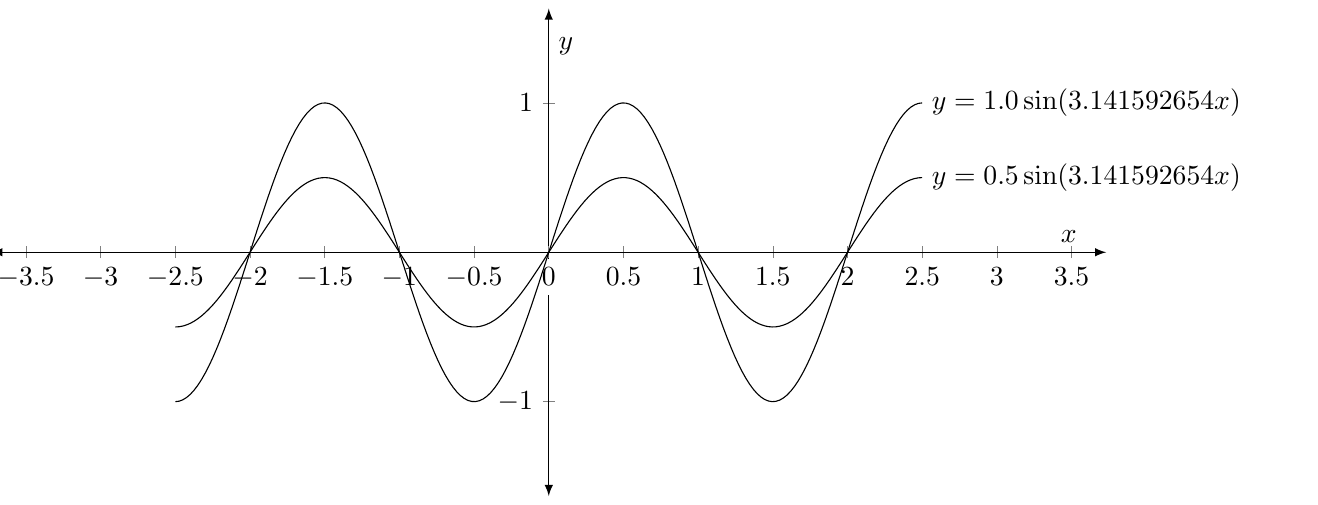
\begin{tikzpicture}
\begin{axis}[width=6in,axis equal image,
          xmax=3,ymax=1.25,
          xmin=-3,ymin=-1.25,
          axis lines=middle,
          enlargelimits,
          axis line style={shorten >=-0.25cm,shorten <=-0.25cm,latex-latex},
          ticklabel style={fill=white},
          extra x ticks={0},
          xlabel=$x$,ylabel=$y$,
          clip=false,
]
\pgfmathsetmacro{\mypi}{pi}
\def\A{1.0}
\def\B{0.5}
\def\k{\mypi}
\def\w{1.5}
\def\t{1.0}
\addplot[domain=-2.5:2.5,mark=none,samples=200] {\A*(sin(deg(\k*x)))} node[fill=white, right]{$y=\A\sin(\k x)$};

\addplot[domain=-2.5:2.5,mark=none,samples=200] {\B*(sin(deg(\k*x)))} node[fill=white, right]{$y=\B\sin(\k x)$};

\end{axis}
\end{tikzpicture}
\label{fig:amplitudes}
\caption{Comparison of two amplitudes}
\end{figure}

%%%%%%%%%%%%%%%%%
\begin{figure}[h!]
\centering
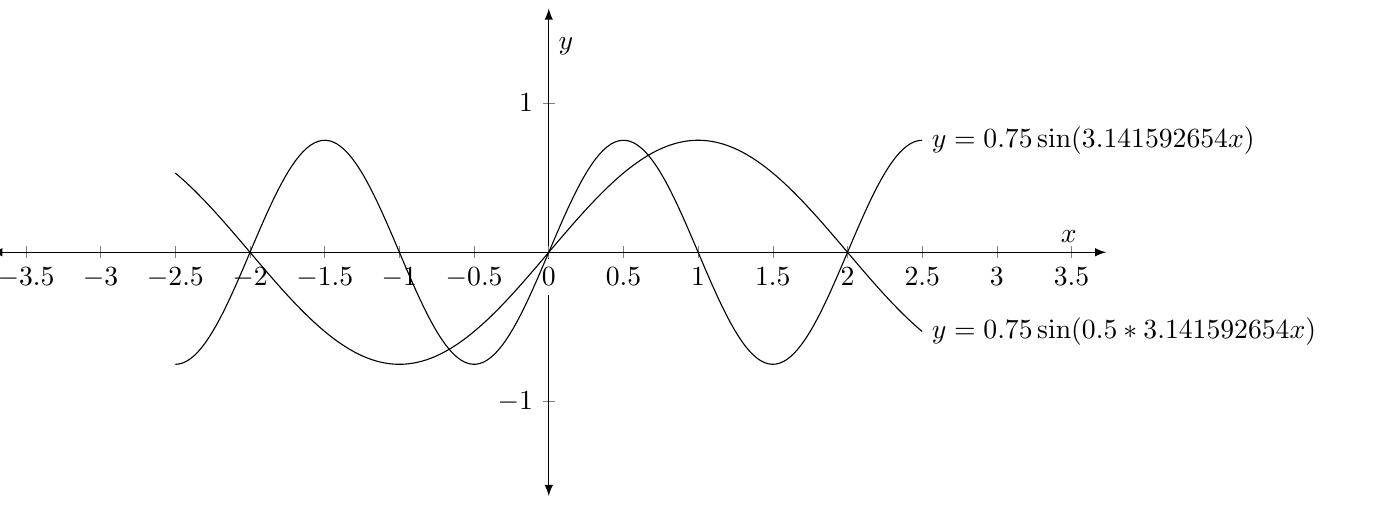
\begin{tikzpicture}
\begin{axis}[width=6in,axis equal image,
          xmax=3,ymax=1.25,
          xmin=-3,ymin=-1.25,
          axis lines=middle,
          enlargelimits,
          axis line style={shorten >=-0.25cm,shorten <=-0.25cm,latex-latex},
          ticklabel style={fill=white},
          extra x ticks={0},
          xlabel=$x$,ylabel=$y$,
          clip=false,
]
\pgfmathsetmacro{\mypi}{pi}
\def\A{0.75}
\def\B{0.5}
\def\k{\mypi}
\def\l{0.5*\mypi}
\def\w{1.5}
\def\t{1.0}
\addplot[domain=-2.5:2.5,mark=none,samples=200] {\A*(sin(deg(\k*x)))} node[fill=white, right]{$y=\A\sin(\k x)$};

\addplot[domain=-2.5:2.5,mark=none,samples=200] {\A*(sin(deg(\l*x)))} node[fill=white, right]{$y=\A\sin(\l x)$};

\end{axis}
\end{tikzpicture}
\label{fig:amplitudes}
\caption{Comparison of two wave numbers}
\end{figure}

%%%%%%%%%%%%%%%%%
\begin{figure}[h!]
\centering
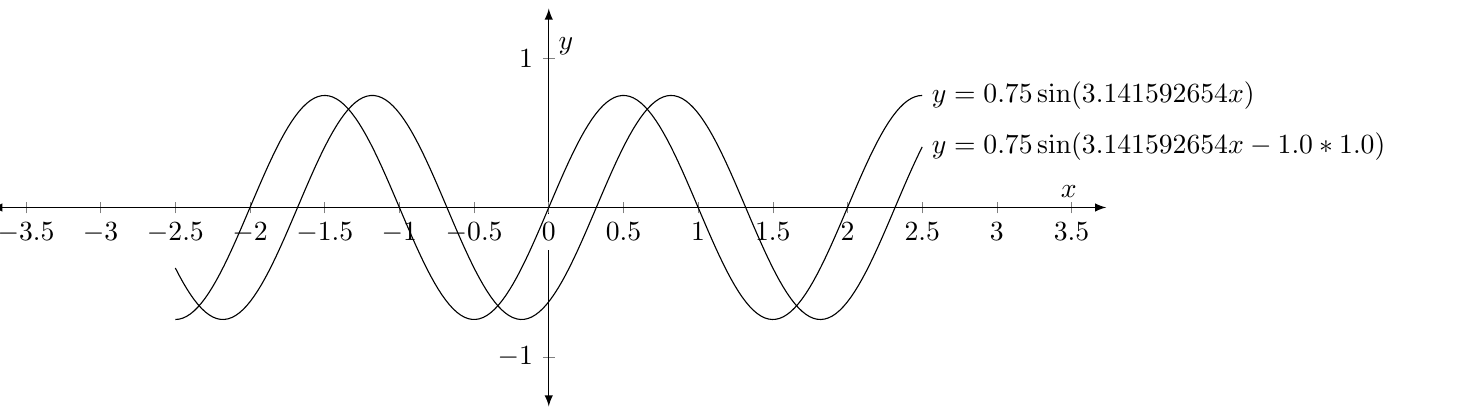
\begin{tikzpicture}
\begin{axis}[width=6in,axis equal image,
          xmax=3,ymax=1.,
          xmin=-3,ymin=-1.,
          axis lines=middle,
          enlargelimits,
          axis line style={shorten >=-0.25cm,shorten <=-0.25cm,latex-latex},
          ticklabel style={fill=white},
          extra x ticks={0},
          xlabel=$x$,ylabel=$y$,
          clip=false,
]
\pgfmathsetmacro{\mypi}{pi}
\def\A{0.75}
\def\B{0.5}
\def\k{\mypi}
\def\l{0.5*\mypi}
\def\w{1.0}
\def\t{1.0}
\addplot[domain=-2.5:2.5,mark=none,samples=200] {\A*(sin(deg(\k*x)))} node[fill=white, right]{$y=\A\sin(\k x)$};

\addplot[domain=-2.5:2.5,mark=none,samples=200] {\A*(sin(deg(\k*x-\w*\t)))} node[fill=white, right]{$y=\A\sin(\k x - \w * \t)$};

%\addplot[domain=-2.5:2.5,mark=none,samples=200] {\A*(sin(deg(\k*x+\w*\t)))} node[fill=white, right]{$y=\A\sin(\k x + \w * \t)$};

\end{axis}
\end{tikzpicture}
\label{fig:amplitudes}
\caption{Comparing an $\omega t$ phase shift}
\end{figure}

\newpage 

\null\vfill 

%https://tex.stackexchange.com/questions/305028/graph-of-pendulum
\begin{figure}[!h]
\centering
\begin{tikzpicture}[scale=2]
    % save length of g-vector and theta to macros
    \pgfmathsetmacro{\Gvec}{1.5}
    \pgfmathsetmacro{\myAngle}{30}
    % calculate lengths of vector components
    \pgfmathsetmacro{\Gcos}{\Gvec*cos(\myAngle)}
    \pgfmathsetmacro{\Gsin}{\Gvec*sin(\myAngle)}
    \coordinate (centro) at (0,0);
    \draw[dashed,gray,-] (centro) -- ++ (0,-2.3) node (mary) [black,below]{$ $};
    \draw[thick] (centro) -- ++(270+\myAngle:3) coordinate (bob);
    \pic [draw, ->, "$\theta$", angle eccentricity=1.5] {angle = mary--centro--bob};
    \draw [blue,thick,-stealth] (bob) -- ($(bob)!\Gcos cm!(centro)$) node[near end, right]{$T$};
    \draw [-stealth] (bob) -- ($(bob)!-\Gcos cm!(centro)$)
      coordinate (gcos)
      node[midway,above right] {$mg\cos\theta$};
    \draw [-stealth] (bob) -- ($(bob)!\Gsin cm!90:(centro)$)
      coordinate (gsin)
      node[midway,above left] {$mg\sin\theta$};
    \draw [-stealth] (bob) -- ++(0,-\Gvec)
      coordinate (g)
      node[near end,left] {$mg$};
    \pic [draw, ->, "$\theta$", angle eccentricity=1.5] {angle = g--bob--gcos};
    \filldraw [fill=black!40,draw=black] (bob) circle[radius=0.1];

\end{tikzpicture}
\end{figure}
\vfill 
\end{document}

%https://tex.stackexchange.com/questions/466502/how-to-print-variable-value-of-draw-function
\newcommand{\xmax}{14}
\newcommand{\fmin}{(pi/3)}
\newcommand{\fmax}{(2*pi)}
\begin{tikzpicture}
[domain=\xmax:0, samples=500]
% The following line uses linear frequency increase
%\draw[ultra thick, red] plot (\x, {sin(deg((\fmin+\x*((\fmax-\fmin))/\xmax)*\x))} );
% The following line uses exponential frequency increase
\draw[ultra thick, red] plot (\x, {sin(deg(exp(ln(\fmin)+\x/\xmax*(ln(\fmax)-ln(\fmin)))*\x))} );
\end{tikzpicture}
\end{document}

Wolfram
plot 1.5*sin(20x-25) AND 1.5*sin(20x-25+10) for 0 < x < 1

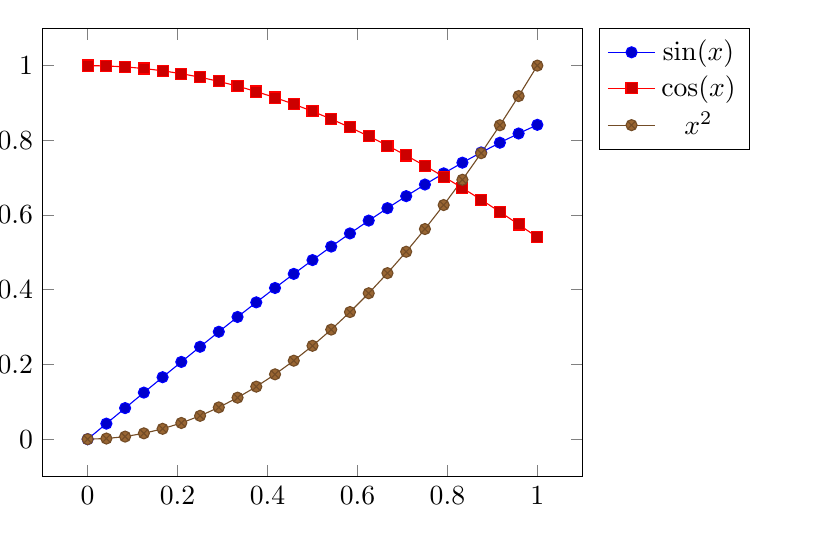
\begin{tikzpicture}
    \begin{axis}[domain=0:1,legend pos=outer north east]
    \addplot {sin(deg(x))}; 
    \addplot {cos(deg(x))}; 
    \addplot {x^2};
    \legend{$\sin(x)$,$\cos(x)$,$x^2$}
    \end{axis}
\end{tikzpicture}

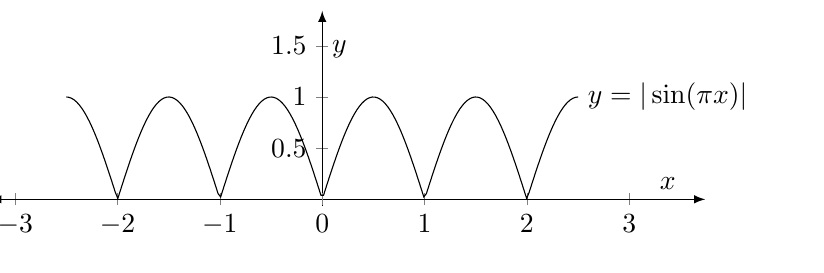
\begin{tikzpicture}
\begin{axis}[width=4in,axis equal image,
          xmax=3,ymax=1.5,
          axis lines=middle,
          enlargelimits,
          axis line style={shorten >=-0.25cm,shorten <=-0.25cm,latex-latex},
          ticklabel style={fill=white},
          extra x ticks={0},
          xlabel=$x$,ylabel=$y$,
          clip=false,
]

\addplot[domain=-2.5:2.5,mark=none,samples=200] {abs(sin(deg(pi*x)))} node[fill=white, right]{$y=\vert\sin(\pi x)\vert$};
\end{axis}
\end{tikzpicture}


\newpage 
\vphantom{}

ARCHIVE

\subheading{Vibrating Springs:} The stiffness of a spring $k$ can be determined experimentally by loading a spring and recording its displacement from its equilibrium position using Hooke's Law, $F_R=-k\triangle y$.

%\begin{minipage}{0.80\textwidth} 
%{\bf Question 6:} A sketch of a mass-loaded spring in static equilibrium is provided in Figure \ref{fig:figure1}. When at rest, the restoring force $F_R$ and the weight $W$ (not Work) and the vertical displacement $\triangle y$ are related. 1) Show for $m=200~g$ and $\triangle y=5~cm$, the spring constant $k=40~N/m$. 2) Using $k=40~N/m$, show also that when set into motion, the period is $T=0.4~s$. Show your work for this question in your lab journal.
%    \vspace{0pt}
%\end{minipage}
%    \hspace{0pt}
%\begin{minipage}{0.20\textwidth}
%    \centering
%\includegraphics[width=0.8\textwidth]{figs/lesson15_spring.png}
%\vspace{0pt}
%\end{minipage}
%%Using the spring apparatus, load the spring with $100~g=0.1~kg$ and record the displacement $\triangle y$ from equilibrium $y_1$ in Table I. Calculate the weight in $Newtons$ and the stiffness constant $k$ in $N/m$. Repeat this procedure for $m=0.15,0.2,0.25,0.3~kg$\footnote{$^*$}{\eightrm Feel free to use different masses and lengths than suggested if it is more convenient. Please indicate any changes in the Tables.}. Plot weight $W$ (ordinate) versus displacement $\triangle y$ (abscissa).% below to discover a nearly linear relationship. Use Excel and its trendline feature to find the slope.

{\bf Experiment:} This experiment will utilize the PHET Masses and Springs simulation found as: 
\vskip 0pt
%\begin{center}
\centerline{\url{https://phet.colorado.edu/en/simulation/masses-and-springs}}
%\end{center}
\vskip 0pt

In this PHET simulation, three springs are hung from overhead, and masses can be selected.
The first experimental goal is to measure the spring constant $k$ of Spring 3 which can be adjusted between a soft and hard stiffness, the slider having 5 indents each way. Select any softness spring 3 setting reporting it as a number between -5 \& 5 below.  Experiment with the simulation, note the movable ruler, dashed line and friction settings. 

What design will establish a reliable numerical value for $k_3$ via experiment. Referencing Fig. \ref{fig:figure1} and Table \ref{tab:table1} work with a partner to populate a similar spreadsheet table with each of the masses $50,100,250,G,Y,R~grams$, here $G,Y,M$ have unknown masses. Hint: consider only static equilibrium cases (allow no motion or friction).

%use your $measured$ $k$ to predict the period of the spring using $T=2\pi\sqrt{\frac{m}{k}}$ where subsequently you will measure and compare $T$. 
%Load the spring with at least five different weights to measure the vertical displacement $\triangle y = y_2 - y_1$. Record this data in Table I.

%See Google Table:
%https://docs.google.com/spreadsheets/d/1GECQiYbnMao4v6mn_K2XHA1UT-9jETrpJHLulby7-Sg/edit#gid=0

\newcolumntype{L}[1]{>{\raggedright\let\newline\\\arraybackslash\hspace{0pt}}m{#1}}  %define column width
\newcolumntype{C}[1]{>{\centering\let\newline\\\arraybackslash\hspace{0pt}}m{#1}}
\newcolumntype{R}[1]{>{\raggedleft\let\newline\\\arraybackslash\hspace{0pt}}m{#1}}
\renewcommand{\arraystretch}{0.9}  %adjust row height

\begin{table}[h]
\begin{minipage}{0.80\textwidth} 
\centering
\captionsetup{width=0.8\textwidth}
\caption{Experimental Data for Spring 3 with softness: \hbox to 30pt{\hrulefill} } \label{tab:table1}
\begin{tabular}{|C{0.3cm}| C{1.4cm}|C{1.6cm}|C{1.7cm}|C{1.2cm}|C{1.2cm}|C{1.4cm}|C{1.3cm}|}\hline 
  & \small Mass ($g$) & \small Mass ($kg$) & \small Weight ($N$) & \small $y_1~(cm)$ & \small $y_2~(cm)$ & \small $\triangle y~(cm)$ &  \small $\triangle y~(m)$ \\ \hline 
0 &  0 & & & & & &  \\ \hline
1 &  & & & & & &  \\ \hline
2 &  & & && & &  \\ \hline
3 &  & & && & &  \\ \hline
4 &  & & && & &  \\ \hline
5 &  & & && & &  \\ \hline
6 & & & && & &  \\ \hline
\end{tabular}

\vspace{0pt}
\end{minipage}
\hspace{0pt}
\begin{minipage}{0.18\textwidth}
\centering
\includegraphics[width=0.9\textwidth]{figs/graph_paper3.png}
\centering
{\it \small Spreadsheet Icon}
\vspace{0pt}
\end{minipage}
\end{table}

{\bf Scatter Plot:} Use your spreadsheet program to build a scatter plot  for spring 3's restoring force $F_R$ ($N$) versus $\triangle y$ ($m$) for your measurements, include the $(0,0)$ point on your graph. Fit the data with a trend line and display both the equation and $R^2$ value in the chart area. What does the trend line slope represent?  Can you and your partner devise a way to establish the three unknown weights ($N$), and thus their masses in $kg$?
\vskip 0pt 

%The slope of $W$ vs $\triangle y$ will be $k$ (recall for $y$ vs $x$, $y=mx+b$). Use Excel's (Google's) trendline feature to determine $k$, which will subsequently be referred to as $k_{measured}$.
%The stiffness of the spring $k$ is independent of the mass in which it supports as long as it is not stretched beyond its designed limits. Determine $k$ for each $m$ using $T=2\pi\sqrt{m\over k}$ and determine the average. 

{\bf Experiment 2:} Now explore the periodic nature of an oscillating spring using spring 3 while preserving your softness spring 3 constant from above. Set any of the masses into a periodic motion using the Stopwatch to determine the period $T$ of the motion; you might find allowing 5 or 10 full cycles easier to count. Recall the period is the amount of time in $seconds$ to complete {\bf one cycle}.  Does the initial displacement before releasing matter? Should you include friction? Collaborate with another to populate a spreadsheet version of Table \ref{tab:table2}.

%Use $k_{measured}$ to predict the time to complete one cycle using $T_{predicted}=2\pi\sqrt{\frac{m}{k_{measured}}}$. 
%From $T_{predicted}$, predict the frequency $f_{predicted}$. 
%Record these in Table \ref{tab:table2} as $T_{predicted}$ and $f_{predicted}$.
%Load the spring apparatus and draw the weight downwards, releasing it to set it into motion. Use a stopwatch to measure the time to complete $10~cycles$ to determine the measured period ($s$) and the frequency ($Hz$).  Compare the $f_{measured}$ to $f_{predicted}$ using $\frac{|f_{predicted}-f_{measured}|}{f_{predicted}}\times 100$. Repeat this procedure for each mass. 
%{\bf Question:} Does an initial displacement of $4~cm$ as compared to $2~cm$ have any bearing on the results?% \hbox to 350pt{\hrulefill}

\begin{table}[h]
\centering
\captionsetup{width=0.8\textwidth}
\caption{Experimental Data for Spring 3 with softness coefficient: \hbox to 30pt{\hrulefill} } \label{tab:table2}
\begin{tabular}{|C{1.0cm}|C{1.1cm}|C{1.0cm}|C{1.33cm}|C{0.8cm}|C{0.8cm}|C{0.8cm}|C{1.4cm}|C{1.4cm}|C{1.4cm}|C{1.2cm}|} \hline 
%
\small Mass ($g$) & \small Mass ($kg$) & \small $k_3$ ($\frac{N}{m}$) & \small $T_{predicted}$ & \small Trial $T_1$ & \small Trial $T_2$ & \small Trial $T_3$ & \small $T^{Average}_{measured}$ & \small $T_{measured}$ \%Error &  \small $T^{2}_{measured}$  & $\frac{m}{k}$ $(\frac{1}{s^2})$  \\ \hline
  0 & & & & & & & & & & \\ \hline
    & & & & & & & & & & \\ \hline
    & & & & & & & & & & \\ \hline
    & & & & & & & & & & \\ \hline
    & & & & & & & & & & \\ \hline
    & & & & & & & & & & \\ \hline
    & & & & & & & & & & \\ \hline 
\end{tabular}
\end{table}

Repeat the experiment for any $T_{measured}$ with $\%Error > 10\%$. Calculate $T^2_{measured}$ from your value of $T^{Average}_{measured}$, and $\frac{m}{k}$. Also determine $f_{measured}$ from $T^{Average}_{measured}$.

{\bf Scatter plot:}  Generate a plot of $T_{measured}$ versus $m/k$, is it linear? Create a second plot of $T^2_{measured}$ versus $m/k$, does the trend line fit of the data seem "more" linear?  What would  the slope of this second plot represent?